\documentclass{standalone}
%\usepackage[subpreambles=true]{standalone}
%\usepackage{xcolor}
\usepackage{latexcolors}
\usepackage{tikz}
\usetikzlibrary{positioning}
\begin{document}
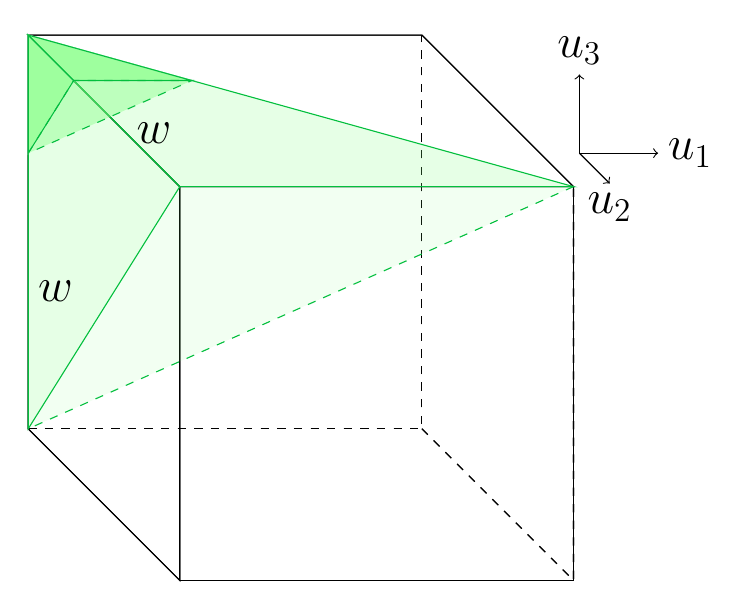
\begin{tikzpicture}[xscale=-1,rotate around x=90,rotate around y=180,rotate around z=0]


\pgfmathsetmacro{\w}{.7}
\pgfmathsetmacro{\a}{5}

\def\labfont{\bfseries\LARGE}
\def\compass{(\a*1.4,0,\a*0.7)}

% draw the compass
\draw[->] \compass -- ++(1,0,0) node[right,font=\labfont] {$u_1$};
\draw[->] \compass -- ++(0,1,0) node[below,font=\labfont] {$u_2$};
\draw[->] \compass -- ++(0,0,1) node[above,font=\labfont] {$u_3$};






% draw the visible cube faces
\draw[black] (0,0,0) -- ++(0,\a,0) -- ++(0,0,\a) -- ++(0,-\a,0) -- cycle;
\draw[black] (0,0,\a) -- ++(\a,0,0) -- ++(0,\a,0) -- ++(-\a,0,0) -- cycle;
\draw[black] (0,\a,0) -- ++(0,0,\a) -- ++(\a,0,0) -- ++(0,0,-\a) -- cycle;
% draw the cube edges
\draw[black,dashed] (0,0,0) --  ++(\a,0,0) -- ++(0,0,\a) ;
\draw[black,dashed] (\a,0,0) --  ++(0,\a,0) -- ++(0,0,\a) ;


\draw[black] (0,0,0) -- ++(0,\a,0) -- ++(0,0,\a) -- ++(0,-\a,0) -- cycle;
\draw[black] (0,0,\a) -- ++(\a,0,0) -- ++(0,\a,0) -- ++(-\a,0,0) -- cycle;
\draw[black] (0,\a,0) -- ++(0,0,\a) -- ++(\a,0,0) -- ++(0,0,-\a) -- cycle;
\draw[black,dashed] (0,0,0) --  ++(\a,0,0) -- ++(0,0,\a) ;
\draw[black,dashed] (\a,0,0) --  ++(0,\a,0) -- ++(0,0,\a) ;

%volume faces
\draw[green!0,fill=green!50,opacity=.2] (0,0,0) --  ++(0,0,\a) -- ++ (0,\a,0) -- cycle;
\draw[green!0,fill=green!50,opacity=.2] (0,0,\a) --  ++(\a,\a,0) --  ++(-\a,0,0) -- cycle ;
\draw[green!0,dashed,fill=green!50,opacity=.1] (\a,\a,\a) --  (0,0,0) --  ++(0,\a,\a) -- cycle;
%volume edges
\draw[darkpastelgreen] (0,0,0) --  ++(0,0,\a) -- ++ (0,\a,0) -- cycle;
\draw[darkpastelgreen] (0,0,\a) --  ++(\a,\a,0) --  ++(-\a,0,0) -- cycle ;
\draw[darkpastelgreen,dashed] (\a,\a,\a) --  (0,0,0);

%polytope faces
\draw[green!0,fill=green!50,opacity=.7] (0,0,\a) -- ++(0,0,-\a+\a*\w) -- ++ (0,\a-\a*\w,\a-\a*\w) -- cycle;
%first point is new, all the rel shifts are similar to volume with coef (1-w)
\draw[green!0,fill=green!50,opacity=.7] (0,0,\a) --  ++(\a-\a*\w,\a-\a*\w,0) --  ++(-\a+\a*\w,0,0) -- cycle ;
\draw[green!0,dashed,fill=green!50,opacity=.4] (0,0,\a*\w) --  ++(0,\a-\a*\w,\a-\a*\w) --  ++ (\a-\a*\w,0,0) -- cycle;

%polytope edges
\draw[darkpastelgreen] (0,0,\a) -- ++(0,0,-\a+\a*\w) -- ++ (0,\a-\a*\w,\a-\a*\w) -- cycle;
%first point is new, all the rel shifts are similar to volume with coef (1-w)
\draw[darkpastelgreen] (0,0,\a) --  ++(\a-\a*\w,\a-\a*\w,0) --  ++(-\a+\a*\w,0,0) -- cycle ;
\draw[darkpastelgreen,dashed] (0,0,\a*\w) --  ++(0,\a-\a*\w,\a-\a*\w) --  ++ (\a-\a*\w,0,0) -- cycle;

\node[right,font=\labfont] at (0,0,0.5*\a*\w) {$w$};
\node[right,font=\labfont] at (0,\a-.5*\a*\w,\a) {$w$};


\end{tikzpicture}
\end{document}